\documentclass[12pt,aspectratio=169]{beamer}

\usetheme[progressbar=frametitle, numbering=fraction]{metropolis}

\usepackage{animate}
\usepackage{multimedia}
\usepackage{xmpmulti}
\usepackage{amsfonts, amsmath, amssymb,latexsym,amsthm, mathrsfs, enumerate, tikz-cd}
\usepackage{hyperref}
\usepackage[all,color]{xy}
\UseCrayolaColors
\usepackage{algorithm}
\usepackage[noend]{algpseudocode}
\usepackage{hyperref}
\usepackage{graphicx} % Allows including images
\usepackage{booktabs} % Allows the use of \toprule, \midrule and \bottomrule in tables
\usepackage[latin1]{inputenc}
\usepackage{epsfig}
\SelectTips{cm}{}

\parskip=5pt
\parindent=15pt
\usepackage{graphicx}
\usepackage{listings}
\numberwithin{equation}{section}
\newtheorem{teo}{Teorema}[section]
\newtheorem*{teo*}{Teorema}
\newtheorem{prop}[teo]{Proposici\'on}
\newtheorem{corol}[teo]{Corolario}
\newtheorem{lema}[teo]{Lema}
\newtheorem{nota}[teo]{Notaci\'on}

\theoremstyle{definition}
\newtheorem{defi}[teo]{Definici\'on}
\newtheorem{prob}[teo]{Problema}
\newtheorem*{sol}{Soluci\'on}
\newtheorem{ex}[teo]{Ejemplo}
\newtheorem{exs}[teo]{Ejemplos}
\newtheorem{obs}[teo]{Observaci\'on}
\newtheorem{obss}[teo]{Observaciones}
\newcommand{\Set}{\mathop{\rm Set}}
\newcommand{\Grp}{\mathop{\rm Grp}}
\newcommand{\Top}{\mathop{\rm Top}}
\newcommand{\Oper}{\mathop{\rm Oper}}

\newenvironment{algoritmo}[1][htb]{%
    \floatname{algorithm}{Algoritmo}% Update algorithm name
   \begin{algorithm}[#1]%
  }{\end{algorithm}}
\renewcommand{\algorithmicrequire}{\textbf{Input:}}
\renewcommand{\algorithmicensure}{\textbf{Output:}}
\newcommand{\Break}{\textbf{break}}
\algblockdefx[ForElse]{ForElse}{EndForElse}{\textbf{else}}{}
\algtext*{EndForElse}

\usepackage{xcolor}
\definecolor{DarkGrey}{HTML}{353535}
\definecolor{ECNURed}{RGB}{164,31,53}
\definecolor{ECNUBrown}{RGB}{134,117,77}
\setbeamercolor{normal text}{ fg= DarkGrey  }
\setbeamercolor{alerted text}{ fg= ECNURed  }
\setbeamercolor{example text}{ fg= ECNUBrown  }
\setbeamercolor{background canvas}{bg=white}
\setbeamertemplate{section in toc}[sections numbered]
\setbeamertemplate{footline}[page number]
\setbeamertemplate{navigation symbols}{}
\setbeamertemplate{blocks}[rounded][shadow=false]
\setbeamertemplate{enumerate items}[default]
\setbeamercolor{block title}{bg=white}
\setbeamercolor{block body}{bg=white}
\setbeamercolor{block title example}{bg=white}
\setbeamercolor{block body example}{bg=white}
\setbeamercolor{block title alerted}{bg=white}
\setbeamercolor{block body alerted}{bg=white}

%----------------------------------------------------------------------------------------
%	TITLE PAGE
%----------------------------------------------------------------------------------------

% \textbf{\LARGE GRADO EN MATEM\'{A}TICAS }
\title[short title]{El producto tensorial de conjuntos dendroidales} % The short title appears at the bottom of every slide, the full title is only on the title page
% \subtitle{Trabajo final de grado}

\author[Roger Brasco] {Roger Brasc\'o Garc\'es}

\institute[NTU] % Your institution as it will appear on the bottom of every slide, may be shorthand to save space
{
    Departamento de Matem\'aticas e Inform\'atica \\
    Universidad de Barcelona % Your institution for the title page
}
\date{9 de Febrero de 2022} % Date, can be changed to a custom date

\titlegraphic{\hfill
\includegraphics[height=1.2cm]{statics/matematiquesinformatica-pos-rgb.png}}


\begin{document}

\begin{frame}
    % Print the title page as the first slide
    \titlepage
\end{frame}

\begin{frame}{Introducci\'on}
    % Throughout your presentation, if you choose to use \section{} and \subsection{} commands, these will automatically be printed on this slide as an overview of your presentation
    \tableofcontents
\end{frame}

%------------------------------------------------
{
% \AtBeginSection{}
\section{Nociones previas}
%------------------------------------------------
\begin{frame}{Nociones previas}
    \begin{itemize}
        \item Categor\'ias
        \item Funtores
        \item Op\'eradas coloreadas
    \end{itemize}
\end{frame}

% \begin{frame}{Categor\'ias}
%     \begin{defi}
%         Una \emph{categor\'{\i}a} $\mathcal{C}$ consiste en:
%         $$
%             \mathcal{C} = ({\rm Ob}(\mathcal{C}), {\rm hom}(\mathcal{C}), \circ, {\rm id})
%         $$
%         % \begin{itemize}
%         %     \item \emph{Objetos}: ${\rm Ob}(\mathcal{C})$.
%         %     % \item Para cada par de objectos $A, B\in{\rm Ob}(\mathcal{C})$ un conjunto $\mathcal{C}(A,B)$ de \emph{morfismos} o \emph{flechas} de $A$ a $B$.
%         %     % \item Para cada tres objectos $A, B, C\in{\rm Ob}(\mathcal{C})$ una \emph{funci\'on de composici\'on}
%         %           $$
%         %               \mathcal{C}(B,C)\times \mathcal{C}(A,B)\stackrel{\circ}{\longrightarrow} \mathcal{C}(A,C)
%         %           $$
%         %           que env\'{\i}a el par $(g,f)$ a $g\circ f$.
%         %     \item Para cada objeto $A$, un elemento ${\rm id}_A\in\mathcal{C}(A,A)$ que llamaremos la \emph{identidad} en $A$.
%         % \end{itemize}
%         Adem\'as, esta estructura cumple los siguientes axiomas:
%         \begin{itemize}
%             \item \emph{Asociatividad}. %La funci\'on de composici\'on es asociativa, esto es, dados $f\in\mathcal{C}(A,B)$, $g\in\mathcal{C}(B,C)$ y $h\in\mathcal{C}(C,D)$, se cumple que $(h\circ g)\circ f=h\circ(g\circ f)$.
%             \item \emph{Unidad}. %La identidad es un elemento neutro para la composici\'on, es decir, para toda $f\in\mathcal{C}(A,B)$ tenemos que $f\circ {\rm id}_A=f={\rm id}_B\circ f$.
%         \end{itemize}
%     \end{defi}

% \end{frame}

% \begin{frame}{Funtores}
%     \begin{defi}
%         Sean $\mathcal{C}$ y $\mathcal{D}$ dos categor\'{\i}as. Un \emph{funtor} $F$ de $\mathcal{C}$ en $\mathcal{D}$, que denotaremos por $F\colon\mathcal{C}\to \mathcal{D}$ consiste en:
%         \begin{itemize}
%             \item Una aplicaci\'on ${\rm Ob}(\mathcal{C})\to {\rm Ob}(\mathcal{D})$. % La imagen de un objeto $A$ de $\mathcal{C}$ la denotaremos por $F(A)$
%             \item Para cada par de objetos $A,B\in\mathcal{C}$ una aplicaci\'on
%                   $$
%                       \mathcal{C}(A,B)\longrightarrow\mathcal{D}(F(A), F(B)).
%                   $$
%                   %   La imagen de un morfismo $f\colon A\to B$ por esta aplicaci\'on la denotaremos por $F(f)\colon F(A)\to F(B)$.
%         \end{itemize}
%         Adem\'as, estas aplicaciones son compatibles con la composici\'on y la unidad. %, esto es, se cumplen los siguientes axiomas:
%         % \begin{itemize}
%         %     \item Dados $f\in\mathcal{C}(A,B)$ y $g\in\mathcal{C}(B,C)$ se cumple que $F(g\circ f)=F(g)\circ F(f)$.
%         %     \item Para todo objeto $A\in\mathcal{C}$ se cumple que $F({\rm id}_A)={\rm id}_{F(A)}$.
%         % \end{itemize}
%     \end{defi}

% \end{frame}

\begin{frame}{Op\'eradas}
    \begin{defi}
        Una \emph{op\'erada} $P$ consiste en una sucesi\'on de conjuntos $\{P(n)\}_{n\ge 0}$ junto con la siguiente estructura:
        \begin{itemize}
            \item Un elemento \emph{unidad} $1\in P(1)$.
            \item Un \emph{producto composici\'on}
                  $$
                      P(n)\times P(k_1) \times\cdots\times P(k_n)\longrightarrow P(k)
                  $$
                  para cada $n$ y $k_1,\dots,k_n$ tal que $k=\sum_{i=1}^{n}{k_i}$.
            \item Para cada $\sigma\in\Sigma_n$ una \emph{acci\'on por la derecha} $\sigma^*\colon P(n)\to P(n)$.
        \end{itemize}
        Adem\'as el producto composici\'on es asociativo, equivariante y compatible con la unidad.
    \end{defi}

\end{frame}

\begin{frame}{Op\'eradas coloreadas}
    % \begin{defi}
    %     Sea $C$ un conjunto. Una \emph{op\'erada $C$-coloreada} $P$ consiste en, para cada $(n+1)$-tupla de colores $(c_1,\ldots,c_n,c)$ con $n\ge 0$, un conjunto $P(c_1,\ldots, c_n;c)$, junto con la siguiente estructura:
    %     \begin{itemize}
    %         \item Un elemento \emph{unidad} $1_c\in P(c;c)$ para cada $c\in C$.
    %         \item Un \emph{producto composici\'on} con $n$ $(n+1)$-tuplas de colores $(c_1,\dots,c_n;c)$.
    %               %   \begin{align*}
    %               %       P(c_1,\dots,c_n;c) & \otimes P(d_{1,1},\dots,d_{1,k_1};c_1) \otimes\dots\otimes P(d_{n,1},\dots,d_{n,k_n};c_n) \\
    %               %                          & \longrightarrow P(d_{1,1},\dots,d_{1,k_1},\dots,d_{n,1},\dots,d_{n,k_n};c)
    %               %   \end{align*}
    %               %   para cada $(n+1)$-tupla de colores $(c_1,\dots,c_n;c)$ y $n$ tuplas cualesquiera
    %               %   $$
    %               %       (d_{1,1},\dots,d_{1,k_1};c_1),\dots,(d_{n,1},\dots,d_{n,k_n};c_n)
    %               %   $$
    %         \item Para cada elemento $\sigma\in\Sigma_n$ una \emph{acci\'on por la derecha} en sus entradas.
    %     \end{itemize}
    %     Adem\'as el producto composici\'on es asociativo, equivariante y compatible con las unidades.
    % \end{defi}
    \begin{defi}
        Sea $P$ una op\'erada $C$-coloreada y $Q$ una op\'erada $D$-coloreada. Un \emph{morfismo de op\'eradas} $f\colon P\to Q$ consiste en una aplicaciones entre los conjuntos de colores $f\colon C\to D$ y aplicaciones
        $$
            f_{c_1,\dots,c_n;c}: P(c_1,\dots,c_n;c) \longrightarrow Q(f(c_1),\dots,f(c_n);f(c))
        $$
        compatibles con el producto composici\'on, las unidades y la acci\'on del grupo sim\'etrico.
    \end{defi}

\end{frame}

%------------------------------------------------
\section{\'Arboles como op\'eradas}
%------------------------------------------------

\begin{frame}{Formalismo de \'arboles}
    Sea $T$ el siguiente \'arbol:
    % Figura arbol + explicación de sus partes %
    $$
        \xy
        <0.08cm, 0cm>:
        %Vertices%
        (0.0, 0.0)*{}="1"; %root_a
        (0.0, 10.0)*=0{\bullet}="2"; %uB
        (-15.0, 20.0)*=0{\bullet}="3"; %vB
        (-22.5, 30.0)*{}="4"; %leaf_e
        (-7.5, 30.0)*{}="5"; %leaf_f
        (0.0, 20.0)*{}="6"; %leaf_c
        (15.0, 20.0)*=0{\bullet}="7"; %wB
        %Edges%
        "1";"2" **\dir{-};
        "2";"3" **\dir{-};
        "3";"4" **\dir{-};
        "3";"5" **\dir{-};
        "2";"6" **\dir{-};
        "2";"7" **\dir{-};
        %Labels%
        (3.0, 9.5)*=0{\scriptstyle r};
        (-11.5, 20.0)*=0{\scriptstyle v};
        (-2.0, 5.0)*=0{\scriptstyle a};
        (-9.5, 14.0)*=0{\scriptstyle b};
        (-21.3, 25.0)*=0{\scriptstyle e};
        (-9, 25.0)*=0{\scriptstyle f};
        (-2.0, 15.0)*=0{\scriptstyle c};
        (10.4, 15.0)*=0{\scriptstyle d};
        (18.0, 20.0)*=0{\scriptstyle w};
        (-13,0)*{T};
        \endxy
    $$
    % La operada $\Omega_p(T)$ tiene seis colores \textit{a, b, c, d, e,} y \textit{f}. Las operaciones generadoras son $v\in \Omega_p(T)(e,f;b)$, $w\in \Omega_p(T)(\_;d)$ y $r\in \Omega_p(T)(b,c,d;a)$.
    % Mientras que las otras operaciones son las operaciones unitarias $1_a,1_b,\dots,1_f$ y las operaciones composici\'on $r\circ_1v\in \Omega_p(T)(e,f,c,d;a)$, $r\circ_2w\in \Omega_p(T)(b,c;a)$ y
    % $$(r\circ_1 v)\circ_3 w = (r\circ_2 w)\circ_1 v  \in \Omega_p(T)(e,f,c;a)$$

\end{frame}
\begin{frame}{\'Arboles como op\'eradas coloreadas}
    \begin{defi}
        Sea $T$ un \'arbol planar con ra\'iz. Denotaremos la op\'erada coloreada no-sim\'etrica generada por $T$ como $\Omega_p(T)$.
        % El conjunto de colores de $\Omega_p(T)$ es el conjunto de aristas $E(T)$ de $T$ y las operaciones est\'an generadas por los v\'ertices del \'arbol.
        % Es decir, para cada v\'ertice $v$ con entradas $e_1,\dots,e_n$ y salida $e$, definimos una operaci\'on $v\in \Omega_p(T)(e_1,\dots,e_n;e)$. Las otras operaciones son las operaciones unitarias y las operaciones obtenidas por composici\'on.
    \end{defi}
    \begin{defi}
        Sea $T$ un \'arbol con ra\'iz. Denotaremos la op\'erada coloreada sim\'etrica generada por $T$ como $\Omega(T)$.
    \end{defi}
    \begin{ex}
        Sea $T$ un \'arbol binario de un solo v\'ertice $v$, entonces $v\in \Omega(T)(b,c;a)$.
    \end{ex}
\end{frame}

\begin{frame}{Categor\'ias \pmb{$\Omega_p$} y \pmb{$\Omega$}}
    \begin{defi}
        La \emph{categor\'ia de \'arboles planares con ra\'iz} $\Omega_p$ es la subcategor\'ia plena de la categor\'ia de op\'eradas coloreadas no-sim\'etricas cuyos objetos son $\Omega_p(T)$ para cada \'arbol $T$.

        % Podemos pensar que $\Omega_p$ es una categor\'ia cuyos objetos son \'arboles planares con ra\'iz.
        % Sean $S$ y $T$ dos \'arboles planares con ra\'iz, el conjunto de morfismos $\Omega_p(S, T)$ es dado por los morfismos entre op\'eradas coloreadas no-sim\'etricas de $\Omega_p(S)$ a $\Omega_p(T)$.
    \end{defi}
    \begin{defi}
        La \emph{categor\'ia de \'arboles con ra\'iz} $\Omega$ es la subcategor\'ia plena de la categor\'ia de op\'eradas coloreadas cuyos objetos son $\Omega(T)$ para todo \'arbol $T$.

        % Podemos pensar que $\Omega$ es una categor\'ia cuyos objetos son \'arboles con ra\'iz.
        % Sean $S$ y $T$ dos \'arboles con ra\'iz, el conjunto de morfismos $\Omega(S, T)$ es dado por los morfismos entre op\'eradas coloreadas de $\Omega(S)$ a $\Omega(T)$.
    \end{defi}
\end{frame}
\begin{frame}{Morfismos en \pmb{$\Omega_p$} y \pmb{$\Omega$}}
    \begin{ex}
        Cara interna
        $$
            \xy
            <0.08cm, 0cm>:
            %Vertices%
            (0.0, 0.0)*{}="1"; %root_a
            (0.0, 10.0)*=0{\bullet}="2"; %uB
            (-22.5, 20.0)*{}="3"; %leaf_e
            (-7.5, 20.0)*{}="4"; %leaf_f
            (7.5, 20.0)*{}="5"; %leaf_c
            (22.5, 20.0)*=0{\bullet}="6"; %wB
            %Edges%
            "1";"2" **\dir{-};
            "2";"3" **\dir{-};
            "2";"4" **\dir{-};
            "2";"5" **\dir{-};
            "2";"6" **\dir{-};
            %Labels%
            (3.0, 9.0)*=0{\scriptstyle u};
            (25.5, 20.0)*=0{\scriptstyle w};
            (-2.0, 5.0)*=0{\scriptstyle a};
            (-13.25, 14.0)*=0{\scriptstyle e};
            (-1, 15.0)*=0{\scriptstyle f};
            (5.75, 15.0)*=0{\scriptstyle c};
            (15.25, 15.0)*=0{\scriptstyle d};
            (-13,0)*{T/b};
            \endxy
            \xy
            <0.08cm, 0cm>:
            (-20, 0.0)*{}="1";
            (20, 0.0)*{}="2";
            (20, 10)*{}="3";
            (-20, 10)*{}="4";
            {\ar(-20, 10)*{};(20,10)*{}};
            (0,13)*{\partial_b};
            \endxy
            \xy
            <0.08cm, 0cm>:
            %Vertices%
            (0.0, 0.0)*{}="1"; %root_a
            (0.0, 10.0)*=0{\bullet}="2"; %uB
            (-15.0, 20.0)*=0{\bullet}="3"; %vB
            (-22.5, 30.0)*{}="4"; %leaf_e
            (-7.5, 30.0)*{}="5"; %leaf_f
            (0.0, 20.0)*{}="6"; %leaf_c
            (15.0, 20.0)*=0{\bullet}="7"; %wB
            %Edges%
            "1";"2" **\dir{-};
            "2";"3" **\dir{-};
            "3";"4" **\dir{-};
            "3";"5" **\dir{-};
            "2";"6" **\dir{-};
            "2";"7" **\dir{-};
            %Labels%
            (3.0, 9.5)*=0{\scriptstyle r};
            (-11.5, 20.0)*=0{\scriptstyle v};
            (-2.0, 5.0)*=0{\scriptstyle a};
            (-9.5, 14.0)*=0{\scriptstyle b};
            (-21.3, 25.0)*=0{\scriptstyle e};
            (-9, 25.0)*=0{\scriptstyle f};
            (-2.0, 15.0)*=0{\scriptstyle c};
            (10.4, 15.0)*=0{\scriptstyle d};
            (18.0, 20.0)*=0{\scriptstyle w};
            (-13,0)*{T};
            \endxy
        $$
    \end{ex}
\end{frame}
%------------------------------------------------
\section{Conjuntos dendroidales}
%------------------------------------------------
\begin{frame}{Conjuntos dendroidales}
    \begin{defi}
        La categor\'ia $dSets$ de \emph{conjuntos dendroidales} es la categor\'ia de prehaces en $\Omega$. Los objetos son funtores $\Omega^{\rm op}\to\Set$ y los morfismos vienen dados por las transformaciones naturales. % La categor\'ia $pd\Set$ de \emph{conjuntos dendroidales planares} esta definida de manera an\'aloga intercambiando $\Omega$ por $\Omega_p$.

        % Un conjunto dendroidal $X$ viene definido como un conjunto $X(T)$, denotado por $X_T$, para cada \'arbol $T$, conjuntamente con una funci\'on $\alpha^{*}\colon X_T \to X_S$ para cada morfismo $\alpha\colon S\to T$ en $\Omega$. Como $X$ es un funtor, entonces $(id)^{*}=id$ y si $\alpha\colon S\to T$ y $\beta\colon R\to S$ son morfismos en $\Omega$, entonces $(\alpha\circ\beta)^{*}=\beta^{*}\circ\alpha^{*}$.

        % El conjunto $X_T$ lo llamaremos conjunto de \emph{d\'endrices con forma T}. %, o simplemente conjunto de $T$-dendrices.

        % Sean $X$ y $Y$ dos conjuntos dendroidales, un \emph{morfismo de conjuntos dendroidales} $f\colon X \to Y$ viene definido por funciones $f\colon X_T\to Y_T$, para cada \'arbol $T$, conmutando con las funciones de estructura. Es decir, si $\alpha\colon S\to T$ es cualquier morfismo en $\Omega$ y $x\in X_T$, entonces $f(\alpha^{*}x)=\alpha^{*}f(x)$.

        % Decimos que $Y$ es un \emph{subconjunto dendroidal} de $X$ si para cada \'arbol $T$ tenemos que $Y_T\subseteq X_T$ y la inclusi\'on $Y \hookrightarrow X$ es un morfismo de conjuntos dendroidales.
    \end{defi}
\end{frame}
\begin{frame}{Nervio dendroidal}
    El funtor $\Omega \to Oper$ que env\'ia un \'arbol $T$ a la op\'erada coloreada $\Omega(T)$ induce, por extensi\'on de Kan, la siguiente adjunci\'on
    \[
        \xymatrix{
            \tau_d\colon dSets\ar@<0.5ex>[r] &  Oper\colon N_d \ar@<0.5ex>[l]
        }
    \]

    El funtor $N_d$ se llama \emph{nervio dendroidal}. Para toda op\'erada $P$, su nervio dendroidal es el conjunto dendroidal
    $$
        N_d(P)_T = Oper(\Omega(T), P)
    $$
    Este funtor es plenamente fiel y $N_d(\Omega(T))=\Omega[T]$ para cada \'arbol $T$ en $\Omega$.
\end{frame}
%------------------------------------------------
\section{Producto tensorial}
%------------------------------------------------

\begin{frame}{Producto tensorial de Boardman--Vogt}
    \begin{defi}
        Sea $P$ una op\'erada sim\'etrica $C$-coloreada, y sea $Q$ una op\'erada sim\'etrica $D$-coloreada. El \emph{producto tensorial de Boardman--Vogt} $P\otimes_{BV}Q$ es una op\'erada $(C\times D)$-coloreada definida en terminos de generadores y relaciones de la siguiente manera.
        Para cada color $d\in D$ y cada operaci\'on $p\in P(c_1,\dots,c_n;c)$ existe un generador
        $$
            p \otimes d \in P\otimes_{BV}Q((c_1,d),\dots,(c_n,d);(c,d))
        $$
        De manera an\'aloga, para cada color $c\in C$ y cada operaci\'on $q\in Q(d_1,\dots,d_m;d)$. % existe un generador
        % $$
        %     c \otimes q \in P\otimes_{BV}Q((c,d_1),\dots,(c,d_m);(c,d))
        % $$
    \end{defi}
\end{frame}
\begin{frame}{Producto tensorial de Boardman--Vogt}
    % Tenemos que las relaciones (i) y (ii) implican que para cada color $d\in D$ la funci\'on $P\to P\otimes_{BV}Q$ es un morfismo de op\'eradas, que viene dada por $p\mapsto p\otimes d$. De manera an\'aloga, tenemos que las relaciones (iii) y (iv) implican que para cada color $c\in C$ la funci\'on $Q\to P\otimes_{BV}Q$ es un morfismo de op\'eradas, que viene dada por $q\mapsto c\otimes q$.

    Estos generadores est\'an sujetos a cinco relaciones:
    \begin{enumerate}
        \item[{\rm (i)}] $(p\otimes d) \circ ((p_1\otimes d),\dots,(p_n\otimes d)) = (p\circ(p_1,\dots,p_n))\otimes d$.
        \item[{\rm (ii)}] $\sigma^{*}(p\otimes d) = (\sigma^{*}p)\otimes d$, para cada $\sigma\in\Sigma_n$.
        \item[{\rm (iii)}] $(c\otimes q) \circ ((c\otimes q_1),\dots,(c\otimes q_m)) = c\otimes (q\circ(q_1,\dots,q_m))$.
        \item[{\rm (iv)}] $\sigma^{*}(c\otimes q) = c\otimes (\sigma^{*}q)$, para cada $\sigma\in\Sigma_m$.
        \item[{\rm (v)}] $\sigma_{n,m}^{*}((p\otimes d)\circ((c_1\otimes q),\dots,(c_n\otimes q))) = (c\otimes q)\circ((p\otimes d_1),\dots,(p\otimes d_m))$, donde $\sigma_{n,m}\in\Sigma_{nm}$ es una permutaci\'on.
              %   Consideramos el conjunto $\Sigma_{nm}$ como el conjunto de biyecciones del conjunto $\{0,1,\dots,nm-1\}$. Cada elemento de dicho conjunto se puede escribir como $kn+j$ de manera \'unica para $0\le k<m$ y $0\le j<n$; y, an\'alogamente, se puede escribir como $km+j$ para $0\le k<n$ y $0\le j<m$.
              %   Finalmente, la permutaci\'on $\sigma_{n,m}$ la definimos de tal manera que $\sigma_{n,m}(kn+j) = jm+k$.
    \end{enumerate}
\end{frame}
\begin{frame}{Relaci\'on de intercambio}
    \begin{ex}
        % Suponemos que $n=2$ y $m=3$.
        % Antes de aplicar la permutaci\'on $\sigma_{2,3}^{*}$
        % Dibujo del arbol (p\otimes d)\circ((c_1\otimes q),\dots,(c_n\otimes q))%
        $$
            \xy
            <0.072cm, 0cm>:
            %Vertices%
            (0.0, 0.0)*{}="1"; %root_c-d
            (0.0, 10.0)*\cir<2pt>{}="2"; %p\otimes dW
            (-45.0, 20.0)*=0{\bullet}="3"; %c_1\otimes qB
            (-75.0, 30.0)*{}="4"; %leaf_c_1-d_1
            (-45.0, 30.0)*{}="5"; %leaf_c_1-d_2
            (-15.0, 30.0)*{}="6"; %leaf_c_1-d_3
            (45.0, 20.0)*=0{\bullet}="7"; %c_2\otimes qB
            (15.0, 30.0)*{}="8"; %leaf_c_2-d_1
            (45.0, 30.0)*{}="9"; %leaf_c_2-d_2
            (75.0, 30.0)*{}="10"; %leaf_c_2-d_3
            %Edges%
            "1";"2" **\dir{-};
            "2";"3" **\dir{-};
            "3";"4" **\dir{-};
            "3";"5" **\dir{-};
            "3";"6" **\dir{-};
            "2";"7" **\dir{-};
            "7";"8" **\dir{-};
            "7";"9" **\dir{-};
            "7";"10" **\dir{-};
            %Labels%
            (5.0, 9.0)*=0{\scriptstyle p\otimes d};
            (-52.0, 19.0)*=0{\scriptstyle c_1\otimes q};
            (52.0, 19.0)*=0{\scriptstyle c_2\otimes q};
            (-5.0, 5.0)*=0{\scriptstyle (c,d)};
            (-20.5, 11.0)*=0{\scriptstyle (c_1,d)};
            (-71.5, 25.0)*=0{\scriptstyle (c_1,d_1)};
            (-45.0, 32.0)*=0{\scriptstyle (c_1,d_2)};
            (-19.0, 25.0)*=0{\scriptstyle (c_1,d_3)};
            (20.5, 11.0)*=0{\scriptstyle (c_2,d)};
            (19.0, 25.0)*=0{\scriptstyle (c_2,d_1)};
            (45.0, 32.0)*=0{\scriptstyle (c_2,d_2)};
            (71.5, 25.0)*=0{\scriptstyle (c_2,d_3)};
            (-13,0)*{T};
            \endxy
        $$

        $$
            \xy
            <0.072cm, 0cm>:
            %Vertices%
            (0.0, 0.0)*{}="1"; %root_c-d
            (0.0, 15.0)*=0{\bullet}="2"; %c\otimes qB
            (-60.0, 30.0)*\cir<2pt>{}="3"; %p\otimes d_1W
            (-75.0, 45.0)*{}="4"; %leaf_c_1-d_1
            (-45.0, 45.0)*{}="5"; %leaf_c_2-d_1
            (0.0, 30.0)*\cir<2pt>{}="6"; %p\otimes d_2W
            (-15.0, 45.0)*{}="7"; %leaf_c_1-d_2
            (15.0, 45.0)*{}="8"; %leaf_c_2-d_2
            (60.0, 30.0)*\cir<2pt>{}="9"; %p\otimes d_3W
            (45.0, 45.0)*{}="10"; %leaf_c_1-d_3
            (75.0, 45.0)*{}="11"; %leaf_c_2-d_3
            %Edges%
            "1";"2" **\dir{-};
            "2";"3" **\dir{-};
            "3";"4" **\dir{-};
            "3";"5" **\dir{-};
            "2";"6" **\dir{-};
            "6";"7" **\dir{-};
            "6";"8" **\dir{-};
            "2";"9" **\dir{-};
            "9";"10" **\dir{-};
            "9";"11" **\dir{-};
            %Labels%
            (5.0, 13.5)*=0{\scriptstyle c\otimes q};
            (-65.5, 30.0)*=0{\scriptstyle p\otimes d_1};
            (6.0, 30.0)*=0{\scriptstyle p\otimes d_2};
            (66, 30.0)*=0{\scriptstyle p\otimes d_3};
            (-4.5, 7.5)*=0{\scriptstyle (c,d)};
            (-32.0, 19.5)*=0{\scriptstyle (c,d_1)};
            (-75, 37.5)*=0{\scriptstyle (c_1,d_1)};
            (-45, 37.5)*=0{\scriptstyle (c_2,d_1)};
            (-5.5, 22.5)*=0{\scriptstyle (c,d_2)};
            (-15, 37.5)*=0{\scriptstyle (c_1,d_2)};
            (15, 37.5)*=0{\scriptstyle (c_2,d_2)};
            (32.0, 19.5)*=0{\scriptstyle (c,d_3)};
            (45, 37.5)*=0{\scriptstyle (c_1,d_3)};
            (75, 37.5)*=0{\scriptstyle (c_2,d_3)};
            (-17,0)*{\sigma_{2,3}^{*}(T)};
            \endxy
        $$
    \end{ex}
\end{frame}
\begin{frame}{Relaci\'on de intercambio}
    \begin{ex}
        % Suponemos que $n=2$ y $m=3$.
        % Antes de aplicar la permutaci\'on $\sigma_{2,3}^{*}$
        % Dibujo del arbol (p\otimes d)\circ((c_1\otimes q),\dots,(c_n\otimes q))%
        $$
            \xy
            <0.072cm, 0cm>:
            %Vertices%
            (0.0, 0.0)*{}="1"; %root_c-d
            (0.0, 10.0)*\cir<2pt>{}="2"; %p\otimes dW
            (-45.0, 20.0)*=0{\bullet}="3"; %c_1\otimes qB
            (-75.0, 30.0)*{}="4"; %leaf_c_1-d_1
            (-45.0, 30.0)*{}="5"; %leaf_c_1-d_2
            (-15.0, 30.0)*{}="6"; %leaf_c_1-d_3
            (45.0, 20.0)*=0{\bullet}="7"; %c_2\otimes qB
            (15.0, 30.0)*{}="8"; %leaf_c_2-d_1
            (45.0, 30.0)*{}="9"; %leaf_c_2-d_2
            (75.0, 30.0)*{}="10"; %leaf_c_2-d_3
            %Edges%
            "1";"2" **\dir{-};
            "2";"3" **[Red]\dir{-};
            "3";"4" **[Blue]\dir{-};
            "3";"5" **[Blue]\dir{-};
            "3";"6" **[Blue]\dir{-};
            "2";"7" **[Red]\dir{-};
            "7";"8" **[Blue]\dir{-};
            "7";"9" **[Blue]\dir{-};
            "7";"10" **[thicker][Blue]\dir{-};
            %Labels%
            (5.0, 9.0)*=0{\scriptstyle p\otimes d};
            (-52.0, 19.0)*=0{\scriptstyle c_1\otimes q};
            (52.0, 19.0)*=0{\scriptstyle c_2\otimes q};
            (-5.0, 5.0)*=0{\scriptstyle (c,d)};
            (-20.5, 11.0)*=0{\scriptstyle (c_1,d)};
            (-71.5, 25.0)*=0{\scriptstyle (c_1,d_1)};
            (-45.0, 32.0)*=0{\scriptstyle (c_1,d_2)};
            (-19.0, 25.0)*=0{\scriptstyle (c_1,d_3)};
            (20.5, 11.0)*=0{\scriptstyle (c_2,d)};
            (19.0, 25.0)*=0{\scriptstyle (c_2,d_1)};
            (45.0, 32.0)*=0{\scriptstyle (c_2,d_2)};
            (71.5, 25.0)*=0{\scriptstyle (c_2,d_3)};
            (-13,0)*{T};
            \endxy
        $$

        $$
            \xy
            <0.072cm, 0cm>:
            %Vertices%
            (0.0, 0.0)*{}="1"; %root_c-d
            (0.0, 15.0)*=0{\bullet}="2"; %c\otimes qB
            (-60.0, 30.0)*\cir<2pt>{}="3"; %p\otimes d_1W
            (-75.0, 45.0)*{}="4"; %leaf_c_1-d_1
            (-45.0, 45.0)*{}="5"; %leaf_c_2-d_1
            (0.0, 30.0)*\cir<2pt>{}="6"; %p\otimes d_2W
            (-15.0, 45.0)*{}="7"; %leaf_c_1-d_2
            (15.0, 45.0)*{}="8"; %leaf_c_2-d_2
            (60.0, 30.0)*\cir<2pt>{}="9"; %p\otimes d_3W
            (45.0, 45.0)*{}="10"; %leaf_c_1-d_3
            (75.0, 45.0)*{}="11"; %leaf_c_2-d_3
            %Edges%
            "1";"2" **\dir{-};
            "2";"3" **[Blue]\dir{-};
            "3";"4" **[Red]\dir{-};
            "3";"5" **[Red]\dir{-};
            "2";"6" **[Blue]\dir{-};
            "6";"7" **[Red]\dir{-};
            "6";"8" **[Red]\dir{-};
            "2";"9" **[Blue]\dir{-};
            "9";"10" **[Red]\dir{-};
            "9";"11" **[Red]\dir{-};
            %Labels%
            (5.0, 13.5)*=0{\scriptstyle c\otimes q};
            (-65.5, 30.0)*=0{\scriptstyle p\otimes d_1};
            (6.0, 30.0)*=0{\scriptstyle p\otimes d_2};
            (66, 30.0)*=0{\scriptstyle p\otimes d_3};
            (-4.5, 7.5)*=0{\scriptstyle (c,d)};
            (-32.0, 19.5)*=0{\scriptstyle (c,d_1)};
            (-75, 37.5)*=0{\scriptstyle (c_1,d_1)};
            (-45, 37.5)*=0{\scriptstyle (c_2,d_1)};
            (-5.5, 22.5)*=0{\scriptstyle (c,d_2)};
            (-15, 37.5)*=0{\scriptstyle (c_1,d_2)};
            (15, 37.5)*=0{\scriptstyle (c_2,d_2)};
            (32.0, 19.5)*=0{\scriptstyle (c,d_3)};
            (45, 37.5)*=0{\scriptstyle (c_1,d_3)};
            (75, 37.5)*=0{\scriptstyle (c_2,d_3)};
            (-17,0)*{\sigma_{2,3}^{*}(T)};
            \endxy
        $$
    \end{ex}
\end{frame}



\begin{frame}{Producto tensorial de conjuntos dendroidales}
    \begin{defi}
        Para todo par de \'arboles $T$ y $S$ en $\Omega$, el \emph{producto tensorial} de los representables $\Omega[T]$ y $\Omega[S]$ se define como
        $$
            \Omega[T]\otimes\Omega[S] = N_d(\Omega(T)\otimes_{BV}\Omega(S))
        $$
        % Donde $N_d$ es el nervio dendroidal, $\Omega(T)$ y $\Omega(S)$ son las op\'eradas coloreadas asociadas a los \'arboles $T$ y $S$, respectivamente; y $\otimes_{BV}$ es el producto tensorial de Boardman--Vogt.

        % Esto define un producto tensorial en toda la categor\'ia de conjuntos dendroidales, ya que es una categor\'ia de prehaces y entonces cada objeto es un col\'imite can\'onico de representables y $\otimes$ conserva col\'imites en cada variable.
    \end{defi}
\end{frame}
\begin{frame}{Producto tensorial de conjuntos dendroidales}
    \begin{defi}
        Sean $X$ e $Y$ dos conjuntos dendroidales y sea $X = \lim_{\to}\Omega[T]$ y $Y = \lim_{\to}\Omega[S]$ sus expresiones can\'onicas como col\'imites de representables. Entonces, definimos el \emph{producto tensorial} $X\otimes Y$ como
        $$
            X\otimes Y = \lim_{\to}\Omega[T]\otimes\lim_{\to}\Omega[S] = \lim_{\to} N_d(\Omega(T)\otimes_{BV}\Omega(S))
        $$
        % Sabemos que este producto tensorial es cerrado gracias a la teor\'ia general de categor\'ias \cite{BCEC}, y el conjunto de $T$-d\'endrices del hom interno viene definido por
        % $$
        %     {\rm Hom}_{dSets}(X,Y)_T = dSets(\Omega[T]\otimes X, Y)
        % $$
        % Para cada par $X$ e $Y$ de conjuntos dendroidales y para cada \'arbol $T$ en $\Omega$.
    \end{defi}
\end{frame}
\begin{frame}{Producto tensorial de conjuntos dendroidales}
    \begin{teo}
        La categor\'ia de conjuntos dendroidales admite una estructura monoidal, sim\'etrica y cerrada. Esta estructura monoidal est\'a \'unicamente determinada (salvo isomorfismo) por la propiedad de que existe un isomorfismo natural
        $$
            \Omega[T]\otimes\Omega[S] \cong N_d(\Omega(T)\otimes_{BV}\Omega(S))
        $$
        para cada par $T$ y $S$ de objetos de $\Omega$. La unidad del producto tensorial es el conjunto dendroidal representable $\Omega[\eta]$, donde $\eta$ es el \'arbol unitario.
    \end{teo}
\end{frame}

%------------------------------------------------
\section{Conjunto de shuffles}
%------------------------------------------------

\begin{frame}{Shuffles}
    \begin{defi}
        Sea $S$ y $T$ dos objetos de $\Omega$. Un \emph{shuffle} de $S$ y $T$ es un \'arbol $R$ cuyo conjunto de aristas es un subconjunto de $E(S)\times E(T)$. La ra\'iz de $R$ es $(a,x)$, donde $a$ es la ra\'iz de $S$ y $x$ es la ra\'iz de $T$,
        y sus hojas son todos los pares $(l_S,l_T)$, donde $l_S$ es una hoja de $S$ y $l_T$ es una hoja de $T$. Los v\'ertices son de la forma
        $$
            \xy
            <0.08cm, 0cm>:
            %Vertices%
            (0.0, 0.0)*{}="1"; %root_b-x
            (0.0, 10.0)*\cir<2pt>{}="2"; %uW
            (-7.5, 20.0)*{}="3"; %leaf_a_1-x
            (7.5, 20.0)*{}="4"; %leaf_a_n-x
            %Edges%
            "1";"2" **\dir{-};
            "2";"3" **\dir{-};
            "2";"4" **\dir{-};
            %Labels%
            (3.0, 10.0)*=0{\scriptstyle u};
            (-5.5, 5)*=0{\scriptstyle (b,\text{ }x)};
            (-10, 13.0)*=0{\scriptstyle (a_1,\text{ }x)};
            (10, 13.0)*=0{\scriptstyle (a_n,\text{ }x)};
            (0,15)*{\dots};
            \endxy
            \xy
            <0.08cm, 0cm>:
            (-15, 0.0)*{}="1";
            (15, 10.0)*{}="2";
            (0,10)*{\rm o};
            \endxy
            \xy
            <0.08cm, 0cm>:
            %Vertices%
            (0.0, 0.0)*{}="1"; %root_a-y
            (0.0, 10.0)*=0{\bullet}="2"; %vB
            (-7.5, 20.0)*{}="3"; %leaf_a-x_1
            (7.5, 20.0)*{}="4"; %leaf_a-x_m
            %Edges%
            "1";"2" **\dir{-};
            "2";"3" **\dir{-};
            "2";"4" **\dir{-};
            %Labels%
            (3.0, 10.0)*=0{\scriptstyle v};
            (-5.5, 5)*=0{\scriptstyle (a,\text{ }y)};
            (-10, 13.0)*=0{\scriptstyle (a,\text{ }x_1)};
            (10, 13.0)*=0{\scriptstyle (a,\text{ }x_m)};
            (0,15)*{\dots};
            \endxy
        $$
        % Donde $u$ es un v\'ertice de $S$ con entradas $a_1,\dots,a_n$ y salida $b$, y $v$ es un v\'ertice de $T$ con entradas $x_1,\dots,x_m$ y salida $y$. Nos referiremos a los dos tipos de v\'ertices como \emph{v\'ertices blancos} y \emph{v\'ertices negros}, respectivamente. Para diferenciarlos visualmente los pintaremos con $\circ$ y $\bullet$, respectivamente.

        % Observamos que existe una biyecci\'on entre los shuffles de dos \'arboles lineales $L_n$ y $L_m$ con los $(n,m)$-shuffles de $[n]\times[m]$.
    \end{defi}
\end{frame}

\begin{frame}{Estructura de orden parcial}
    Existen los \emph{shuffles intermediarios} $R_k$ $(1 < k < N)$ entre $R_1$ y $R_N$. % obtenidos filtrando los v\'ertices negros en $R_1$ hacia la ra\'iz del \'arbol mediante intercambios con los v\'ertices blancos.
    % Todo $R_k$ se obtiene desde un $R_l$ anterior. Es decir, cada intercambio se basa en transformar una configuraci\'on de $R_l$
    $$
        \xy
        <0.075cm, 0cm>:
        %Vertices%
        (0.0, 0.0)*{}="1"; %root_a-x
        (0.0, 15.0)*\cir<2pt>{}="2"; %0W
        (-25.0, 30.0)*=0{\bullet}="3"; %1B
        (-37.5, 45.0)*{}="4"; %leaf_b_1-y_1
        (-12.5, 45.0)*{}="5"; %leaf_b_n-y_1
        (25.0, 30.0)*=0{\bullet}="6"; %2B
        (12.5, 45.0)*{}="7"; %leaf_b_1-y_m
        (37.5, 45.0)*{}="8"; %leaf_b_n-y_m
        %Edges%
        "1";"2" **\dir{-};
        "2";"3" **\dir{-};
        "3";"4" **\dir{-};
        "3";"5" **\dir{-};
        "2";"6" **\dir{-};
        "6";"7" **\dir{-};
        "6";"8" **\dir{-};
        %Labels%
        (-5.5, 7.5)*=0{\scriptstyle (a,\text{ }x)};
        (-19.5, 21)*=0{\scriptstyle (a,\text{ }y_1)};
        (-39, 37.5)*=0{\scriptstyle (b_1,\text{ }y_1)};
        (-11, 37.5)*=0{\scriptstyle (b_n,\text{ }y_1)};
        (19.5, 21)*=0{\scriptstyle (a,\text{ }y_m)};
        (10.5, 37.5)*=0{\scriptstyle (b_1,\text{ }y_m)};
        (39.5, 37.5)*=0{\scriptstyle (b_n,\text{ }y_m)};
        (-25,35)*{\dots};
        (25,35)*{\dots};
        (0,20)*{\dots\dots};
        (-13,0)*{R_l};
        \endxy
        \xy
        <0.08cm, 0cm>:
        (-10, 0.0)*{}="1";
        (10, 10.0)*{}="2";
        {\ar(-10, 10)*{};(10,10)*{}};
        \endxy
        \xy
        <0.075cm, 0cm>:
        %Vertices%
        (0.0, 0.0)*{}="1"; %root_a-x
        (0.0, 15.0)*=0{\bullet}="2"; %0B
        (-25.0, 30.0)*\cir<2pt>{}="3"; %1W
        (-37.5, 45.0)*{}="4"; %leaf_b_1-y_1
        (-12.5, 45.0)*{}="5"; %leaf_b_1-y_m
        (25.0, 30.0)*\cir<2pt>{}="6"; %2W
        (12.5, 45.0)*{}="7"; %leaf_b_n-y_1
        (37.5, 45.0)*{}="8"; %leaf_b_n-y_m
        %Edges%
        "1";"2" **\dir{-};
        "2";"3" **\dir{-};
        "3";"4" **\dir{-};
        "3";"5" **\dir{-};
        "2";"6" **\dir{-};
        "6";"7" **\dir{-};
        "6";"8" **\dir{-};
        %Labels%
        (-5.5, 7.5)*=0{\scriptstyle (a,\text{ }x)};
        (-19.5, 21)*=0{\scriptstyle (b_1,\text{ }x)};
        (-39, 37.5)*=0{\scriptstyle (b_1,\text{ }y_1)};
        (-11, 37.5)*=0{\scriptstyle (b_1,\text{ }y_m)};
        (19.5, 21)*=0{\scriptstyle (b_n,\text{ }x)};
        (10.5, 37.5)*=0{\scriptstyle (b_n,\text{ }y_1)};
        (39.5, 37.5)*=0{\scriptstyle (b_n,\text{ }y_m)};
        (-25,35)*{\dots};
        (25,35)*{\dots};
        (0,20)*{\dots\dots};
        (-13,0)*{R_k};
        \endxy
    $$

    Si un shuffle $R_k$ se obtiene de otro shuffle $R_l$ mediante la norma de arriba, entonces $R_l\le R_k$.
\end{frame}

\begin{frame}{Producto tensorial de \'arboles}
    \begin{lema}
        Para todo shuffle $R_i$ de $S$ y $T$ tenemos un monomorfismo
        $$
            \xymatrix{
                m\colon\Omega[R_i] \ar@{>->}[r] & \Omega[S]\otimes\Omega[T]
            }
        $$
        % El subconjunto dendroidal, que viene dado por la im\'agen de este monomorfismo, lo denotaremos $m(R_i)$.
    \end{lema}
    % \begin{proof}
    %     Los v\'ertices del conjunto dendroidal $\Omega[R_i]$ son las aristas del \'arbol $R_i$. La funci\'on $m$ env\'ia aristas nombradas como $(a, x)$ en $R_i$ a la arista con el mismo nombre en $\Omega[S]\otimes\Omega[T]$.
    %     Un morfismo $\Omega[R]\to X$, de un representable de un conjunto dendroidal a un conjunto dendroidal arbitrario, es un monomorfismo desde que el morfismo $\Omega[R]_\eta \to X_\eta$ lo es en los v\'ertices.

    % \end{proof}
    \begin{corol}
        Para todo objeto $T$ y $S$ en $\Omega$, tenemos que
        $$
            \Omega[S]\otimes\Omega[T] = \bigcup_{i=1}^{N} m(R_i)
        $$
        % donde la uni\'on recorre todos los posibles shuffles de $S$ y $T$.
    \end{corol}
\end{frame}
\begin{frame}{N\'umero de shuffles}
    \begin{prop}
        El n\'umero de shuffles $sh(S,\text{ }T)$ de dos \'arboles $S$ y $T$ satisface tres propiedades:
        \begin{enumerate}
            \item[{\rm (i)}] Sim\'etrico: $sh(S, \text{ }T) = sh(T, \text{ }S)$
            \item[{\rm (ii)}] Unitario: Si $T$ es un \'arbol unitario $\eta$, entonces $sh(S, \text{ }\eta)=1$
            \item[{\rm (iii)}] Inducci\'on: Si $S=C_n[S_1,\dots,S_n]$ y $T=C_m[T_1,\dots,T_m]$, entonces
                  $$
                      sh(S, \text{ }T)  = \prod_{i=1}^n sh(S_i, \text{ }T) + \prod_{j=1}^m sh(S, \text{ }T_j)
                  $$
        \end{enumerate}
        % donde $C_n$ y $C_m$ son $n$ y $m$-corolas, respectivamente; y $C_n[S_1,\dots,S_n]$ es una $n$-corola que cada hoja $i$-esima la conectamos con la ra\'iz del \'arbol $S_i$. \cite[Proposici\'on 3.1]{SoT}.
    \end{prop}
\end{frame}

\begin{frame}{Generar shuffles en Python}
    \begin{ex}
        Sean $S$ y $T$ los \'arboles
        $$
            \xy
            <0.08cm, 0cm>:
            %Vertices%
            (0.0, 0.0)*{}="1"; %root_a
            (0.0, 10.0)*\cir<2pt>{}="2"; %0W
            (-22.5, 20.0)*\cir<2pt>{}="3"; %1W
            (-37.5, 30.0)*{}="4"; %leaf_d
            (-22.5, 30.0)*{}="5"; %leaf_e
            (-7.5, 30.0)*{}="6"; %leaf_f
            (22.5, 20.0)*\cir<2pt>{}="7"; %2W
            (7.5, 30.0)*{}="8"; %leaf_g
            (22.5, 30.0)*{}="9"; %leaf_h
            (37.5, 30.0)*{}="10"; %leaf_i
            %Edges%
            "1";"2" **\dir{-};
            "2";"3" **\dir{-};
            "3";"4" **\dir{-};
            "3";"5" **\dir{-};
            "3";"6" **\dir{-};
            "2";"7" **\dir{-};
            "7";"8" **\dir{-};
            "7";"9" **\dir{-};
            "7";"10" **\dir{-};
            (-13,0)*{S};
            \endxy
            \xy
            <0.08cm, 0cm>:
            (-10, 0.0)*{}="1";
            (10, 10.0)*{}="2";
            \endxy
            \xy
            <0.08cm, 0cm>:
            %Vertices%
            (0.0, 0.0)*{}="1"; %root_a
            (0.0, 10.0)*=0{\bullet}="2"; %0B
            (-15.0, 20.0)*=0{\bullet}="3"; %1B
            (-15.0, 30.0)*=0{\bullet}="4"; %3B
            (-22.5, 40.0)*{}="5"; %leaf_f
            (-7.5, 40.0)*{}="6"; %leaf_g
            (15.0, 20.0)*=0{\bullet}="7"; %2B
            (15.0, 30.0)*=0{\bullet}="8"; %4B
            (7.5, 40.0)*{}="9"; %leaf_h
            (22.5, 40.0)*{}="10"; %leaf_i
            %Edges%
            "1";"2" **\dir{-};
            "2";"3" **\dir{-};
            "3";"4" **\dir{-};
            "4";"5" **\dir{-};
            "4";"6" **\dir{-};
            "2";"7" **\dir{-};
            "7";"8" **\dir{-};
            "8";"9" **\dir{-};
            "8";"10" **\dir{-};
            (-13,0)*{T};
            \endxy
        $$
    \end{ex}
\end{frame}
\begin{frame}{Generar shuffles en Python}
    El conjunto de shuffles resultante ser\'ia
    \begin{center}\makebox[0pt]{
            \movie{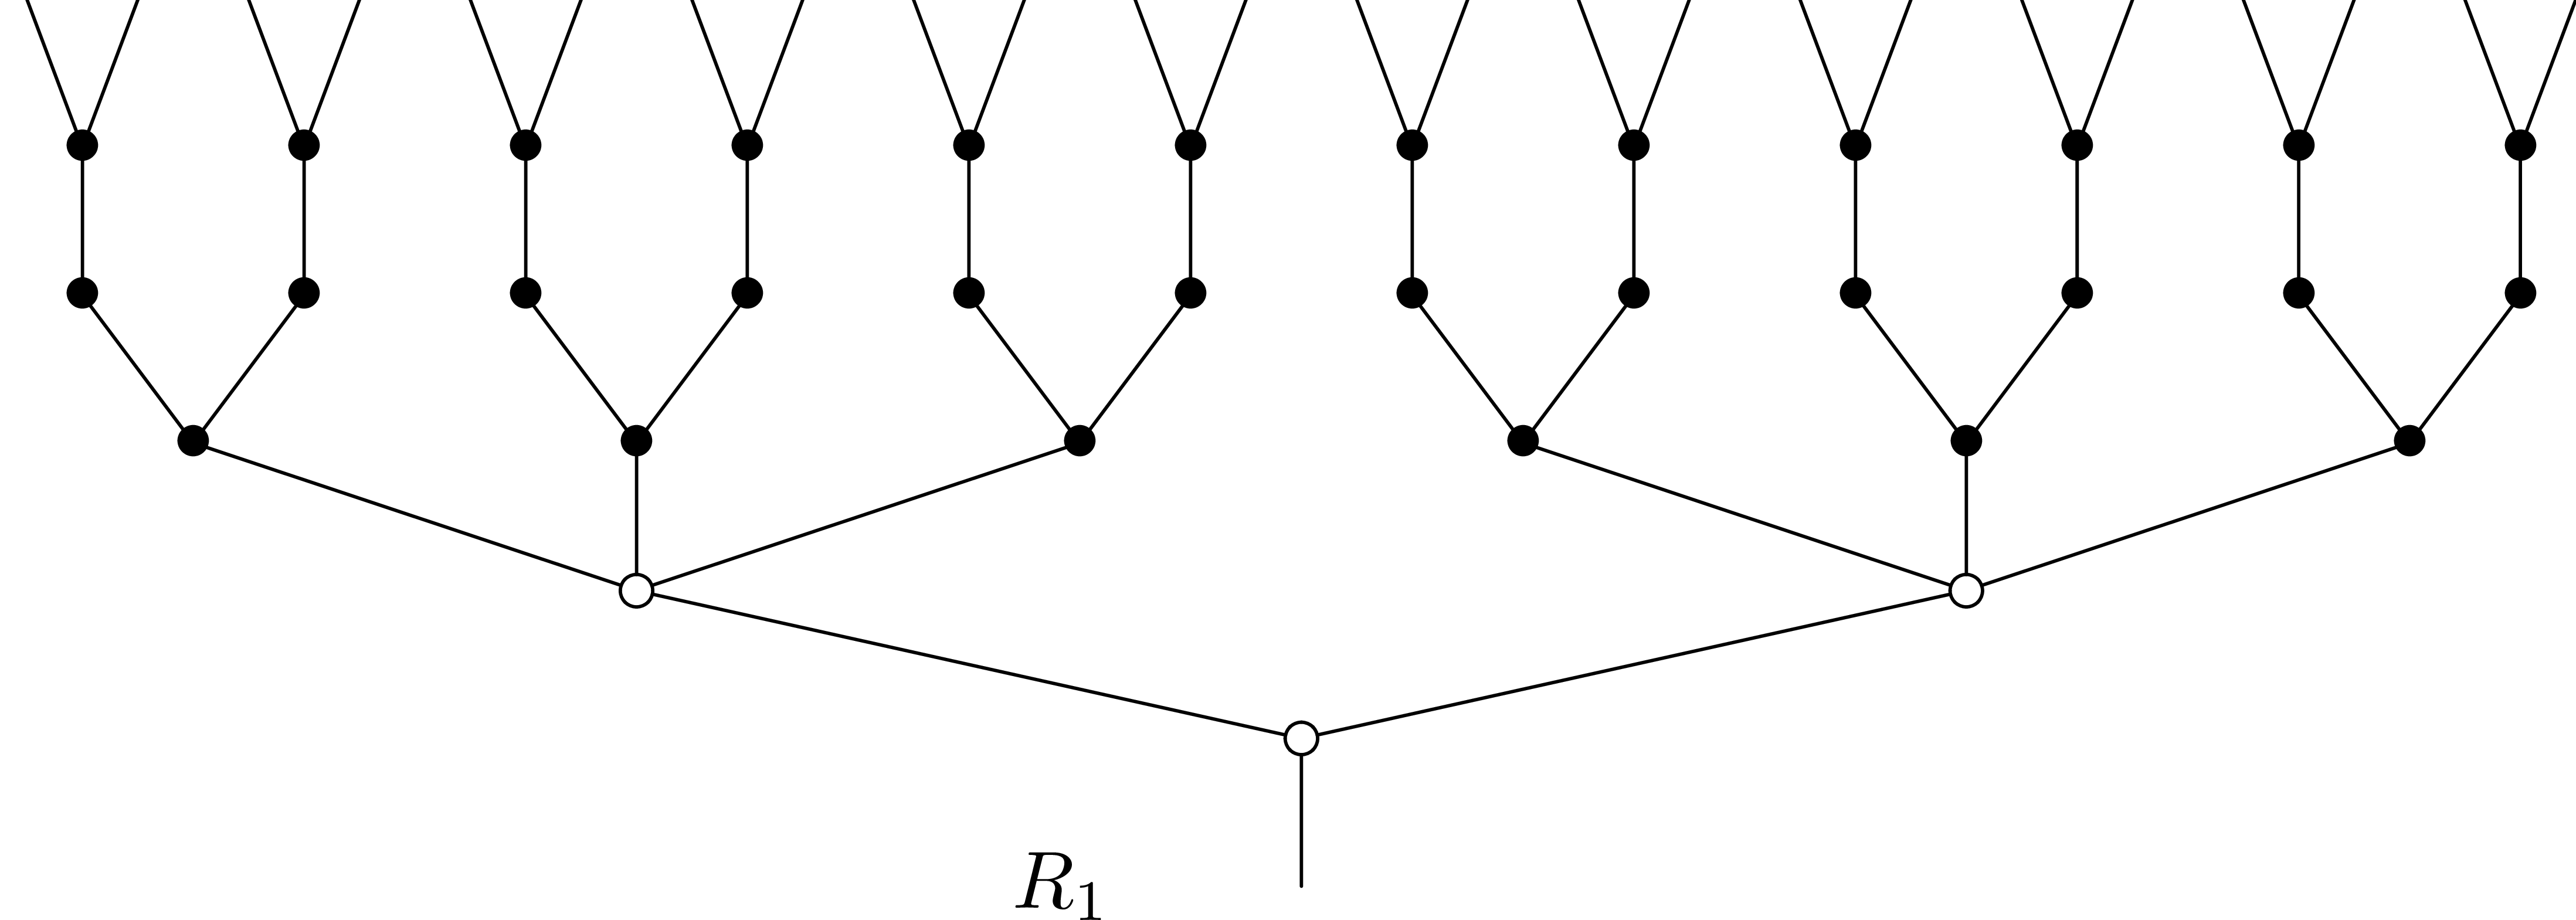
\includegraphics{statics/R1.png}}{statics/slow.avi}
        }\end{center}

\end{frame}
}
%------------------------------------------------
% \section{Conclusiones}
%------------------------------------------------

% \begin{frame}{Conclusiones}
%     H
% \end{frame}

%------------------------------------------------

\begin{frame}
    \Huge{\centerline{\textbf{Gracias por vuestra atenci\'on}}}
\end{frame}

%----------------------------------------------------------------------------------------

\end{document}